\documentclass[tikz,border=3pt]{standalone}
\usepackage{mathptmx}
\usepackage{amsmath}
\usetikzlibrary{arrows.meta,calc}
\definecolor{pvblue}{HTML}{0072B2}
\definecolor{pvorange}{HTML}{D55E00}
\definecolor{pvink}{HTML}{374151}
\definecolor{pvmuted}{HTML}{9AA5B1}
\begin{document}
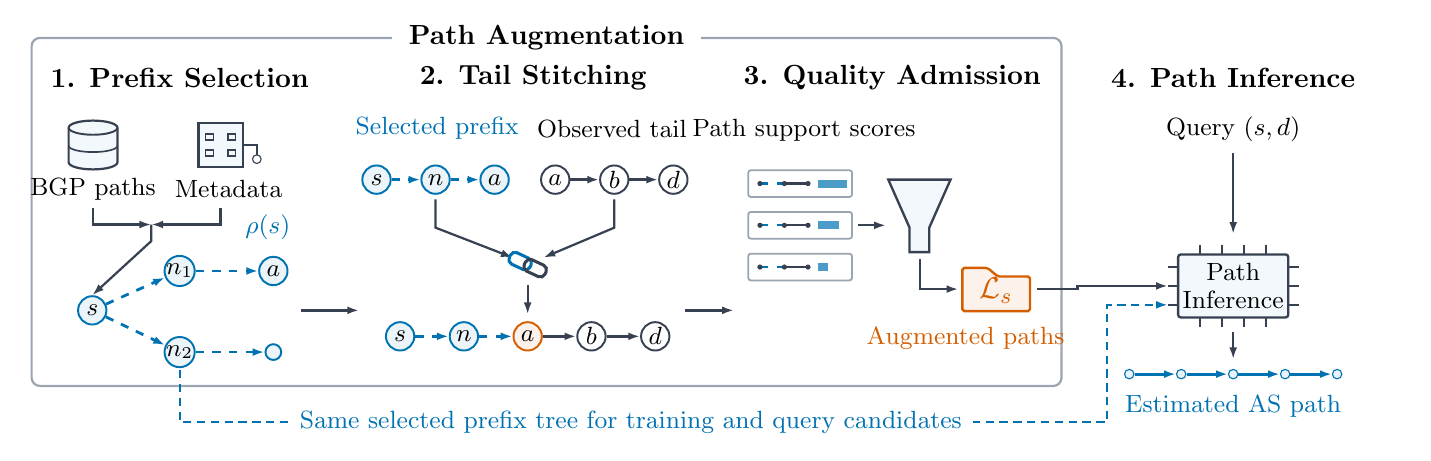
\begin{tikzpicture}[
 font=\fontsize{9.1}{10.3}\selectfont,
 >={Latex[length=1.5mm,width=1mm]},
 flow/.style={->,draw=pvink,line width=.8pt},
 prefixedge/.style={->,draw=pvblue,line width=1pt,dashed},
 observededge/.style={->,draw=pvink,line width=1pt},
 heading/.style={font=\fontsize{10}{11.3}\selectfont\bfseries,align=center,inner sep=0pt},
 label/.style={align=center,inner sep=0pt},
 as/.style={circle,draw=pvink,fill=white,line width=.7pt,
  minimum size=.36cm,inner sep=0pt,font=\fontsize{9}{10}\selectfont},
 selected/.style={as,draw=pvblue,fill=pvblue!8},
 pics/database/.style={code={
  \path[draw=pvink,fill=pvblue!5,line width=.8pt]
   (-.31,.22)--(-.31,-.22) arc[start angle=180,end angle=360,x radius=.31,y radius=.09]
   --(.31,.22) arc[start angle=0,end angle=180,x radius=.31,y radius=.09];
  \draw[pvink,line width=.7pt] (-.31,.22) arc[start angle=180,end angle=360,x radius=.31,y radius=.09];
  \draw[pvink,line width=.6pt] (-.31,-.01) arc[start angle=180,end angle=360,x radius=.31,y radius=.08];
 }},
 pics/metadata/.style={code={
  \draw[pvink,fill=pvblue!5,line width=.8pt] (-.28,-.28) rectangle (.28,.28);
  \foreach \x in {-.14,.14} {\foreach \y in {-.10,.10} {
   \draw[pvink,line width=.6pt] (\x-.05,\y-.04) rectangle (\x+.05,\y+.04);}}
  \draw[pvink,line width=.65pt] (.28,0)--(.46,0)--(.46,-.18);
  \draw[pvink,fill=white] (.46,-.18) circle (.055);
 }},
 pics/library/.style={code={
  \path[draw=pvorange,fill=pvorange!8,line width=.85pt,rounded corners=.7pt]
   (-.43,-.28)--(-.43,.27)--(-.11,.27)--(.02,.16)--(.43,.16)--(.43,-.28)--cycle;
  \node[text=pvorange,font=\fontsize{11}{12}\selectfont] at (0,-.02) {$\mathcal L_s$};
 }},
 pics/chip/.style={code={
  \draw[pvink,fill=pvblue!5,line width=.85pt,rounded corners=1pt]
   (-.70,-.40) rectangle (.70,.40);
  \foreach \x in {-.42,-.14,.14,.42} {
   \draw[pvink,line width=.7pt] (\x,.40)--(\x,.52) (\x,-.40)--(\x,-.52);}
  \foreach \y in {-.24,0,.24} {
   \draw[pvink,line width=.7pt] (-.70,\y)--(-.83,\y) (.70,\y)--(.83,\y);}
  \node[align=center,font=\fontsize{9.2}{10.3}\selectfont] {Path\\Inference};
 }},
 pics/link/.style={code={
  \draw[pvblue,line width=1.1pt,rotate=-25,rounded corners=1.8pt]
   (-.25,-.08) rectangle (.04,.08);
  \draw[pvink,line width=1.1pt,rotate=-25,rounded corners=1.8pt]
   (-.04,-.08) rectangle (.25,.08);
 }}
]
\path[use as bounding box] (-.25,-1.08) rectangle (17.22,4.07);
% The augmentation boundary includes prefix selection, construction, admission.
\draw[pvmuted,line width=.8pt,rounded corners=3pt]
 (-.20,-.48) rectangle (12.88,3.94);
\node[heading,fill=white,inner xsep=6pt] at (6.34,3.94) {Path Augmentation};
\node[heading] at (1.68,3.43) {1. Prefix Selection};
\node[heading] at (6.17,3.43) {2. Tail Stitching};
\node[heading] at (10.73,3.43) {3. Quality Admission};
\node[heading] at (15.06,3.43) {4. Path Inference};

% Public evidence and a compact branching picture.
\pic at (.58,2.58) {database};
\pic at (2.20,2.58) {metadata};
\node[label] at (.58,2.02) {BGP paths};
\node[label] at (2.30,2.02) {Metadata};
\draw[flow] (.58,1.78)--(.58,1.57)--(1.32,1.57);
\draw[flow] (2.20,1.78)--(2.20,1.57)--(1.32,1.57);
\node[label,text=pvblue] at (2.80,1.53) {$\rho(s)$};
\node[selected] (s) at (.57,.48) {$s$};
\node[selected] (n1) at (1.68,.98) {$n_1$};
\node[selected] (n2) at (1.68,-.05) {$n_2$};
\node[selected] (a1) at (2.87,.98) {$a$};
\node[selected,minimum size=.20cm] (a2) at (2.87,-.05) {};
\draw[flow] (1.32,1.57)--(1.32,1.36)--(s.north);
\draw[prefixedge] (s)--(n1); \draw[prefixedge] (s)--(n2);
\draw[prefixedge] (n1)--(a1); \draw[prefixedge] (n2)--(a2);
\draw[flow,line width=1pt] (3.22,.48)--(3.96,.48);

% Learned source prefixes reuse real observed tails at a shared anchor.
\node[label,text=pvblue] at (4.95,2.79) {Selected prefix};
\node[label] at (7.17,2.79) {Observed tail};
\node[selected] (ps) at (4.18,2.14) {$s$};
\node[selected] (pn) at (4.93,2.14) {$n$};
\node[selected] (pa) at (5.68,2.14) {$a$};
\node[as] (ta) at (6.45,2.14) {$a$};
\node[as] (tb) at (7.20,2.14) {$b$};
\node[as] (td) at (7.95,2.14) {$d$};
\draw[prefixedge] (ps)--(pn); \draw[prefixedge] (pn)--(pa);
\draw[observededge] (ta)--(tb); \draw[observededge] (tb)--(td);
\draw[flow] (4.93,1.89)--(4.93,1.53)--(5.91,1.15);
\draw[flow] (7.20,1.89)--(7.20,1.53)--(6.30,1.15);
\pic at (6.10,1.06) {link};
\draw[flow] (6.10,.80)--(6.10,.43);
\node[selected] (js) at (4.48,.15) {$s$};
\node[selected] (jn) at (5.29,.15) {$n$};
\node[as,draw=pvorange,fill=pvorange!8] (ja) at (6.10,.15) {$a$};
\node[as] (jb) at (6.91,.15) {$b$};
\node[as] (jd) at (7.72,.15) {$d$};
\draw[prefixedge] (js)--(jn); \draw[prefixedge] (jn)--(ja);
\draw[observededge] (ja)--(jb); \draw[observededge] (jb)--(jd);
\draw[flow,line width=1pt] (8.10,.48)--(8.72,.48);

% Complete-path scores feed a single source-relative quality gate.
\node[label] at (9.61,2.77) {Path support scores};
\foreach \y/\bar in {2.09/.37,1.56/.27,1.03/.12} {
 \begin{scope}[shift={(9.56,\y)}]
  \draw[pvmuted,fill=white,rounded corners=1pt,line width=.65pt] (-.66,-.17) rectangle (.66,.17);
  \draw[pvblue,dashed,line width=.8pt] (-.51,0)--(-.20,0);
  \draw[pvink,line width=.8pt] (-.20,0)--(.10,0);
  \foreach \x in {-.51,-.20,.10} {\fill[pvink] (\x,0) circle (.033);}
  \fill[pvblue!70] (.23,-.05) rectangle ({.23+\bar},.05);
 \end{scope}
}
\draw[flow] (10.30,1.56)--(10.65,1.56);
\path[draw=pvink,fill=pvblue!5,line width=.85pt]
 (10.68,2.14)--(11.47,2.14)--(11.20,1.53)--(11.20,1.22)--(10.95,1.22)--(10.95,1.53)--cycle;
\draw[flow] (11.08,1.13)--(11.08,.75)--(11.57,.75);
\pic at (12.05,.75) {library};
\node[label,text=pvorange] at (11.66,.13) {Augmented paths};
\draw[flow,line width=1pt] (12.57,.75)--(13.08,.75)--(13.08,.79)--(14.23,.79);


% Query candidates and training share exactly the selected source tree.
\node[label] at (15.06,2.78) {Query $(s,d)$};
\draw[flow] (15.06,2.48)--(15.06,1.45);
\pic at (15.06,.79) {chip};
\draw[flow] (15.06,.20)--(15.06,-.14);
\foreach \x [count=\i] in {13.74,14.40,15.06,15.72,16.38} {
 \node[circle,draw=pvblue,fill=pvblue!9,minimum size=.12cm,inner sep=0pt] (out\i) at (\x,-.33) {};
}
\foreach \i/\j in {1/2,2/3,3/4,4/5} {\draw[pvblue,line width=1pt,->] (out\i)--(out\j);}
\node[label,text=pvblue] at (15.06,-.74) {Estimated AS path};
\draw[->,pvblue,line width=.8pt,dash pattern=on 3pt off 2pt]
 (1.68,-.28)--(1.68,-.94)--(13.46,-.94)--(13.46,.55)--(14.23,.55);
\node[label,fill=white,inner xsep=4pt,text=pvblue] at (7.41,-.94)
 {Same selected prefix tree for training and query candidates};
\end{tikzpicture}
\end{document}
